\clearpage{\pagestyle{empty}\cleardoublepage}

\chapter{\wbx\ analysis: search configuration}\label{app:wbx_statanalyses}

In the 7~\tev\ analysis
described in Appendix~\ref{app:wbx7tev},
three configurations have been tested to derive the final
results of this search: \loose\ selection using
$m_{\rm reco}$ (see Figure~\ref{fig:mrecoLOOSEBIS}) 
and profiling of overall $t\bar{t}$ yield (``\loose''); \tight\ selection 
using $m_{\rm reco}$ (see Figure~\ref{fig:mrecoTIGHTBIS})
(``\tight''); \tight\ selection  considering just the overall yield and not 
the shape of $m_{\rm reco}$ (``\tight\ cut-and-count'').
The expected value of $CL_{\rm s}$ (see Section~\ref{sec:cls})
as a function of $m_{\T}$ is
used to choose the best performing strategy.
As was shown in Table~\ref{tab:SystSummary}, the prediction for 
the $t\bar{t}$ background is affected by 
large systematic uncertainties originating from \btag ged jet 
identification efficiency, 
jet energy calibration and resolution and physics modeling in the Monte
Carlo generators. 
In the case of the \loose\ selection configuration the low-mass sideband
region dominated by $t\bar{t}$ can be used to exploit the available data 
statistics to reduce the degrading 
impact of systematic uncertainties on the sensitivity of the search. 
This is accomplished by fitting, during the statistical analysis,
a single nuisance parameter representing a scaling factor on 
the overall $t\bar{t}$ yield. Such procedure is
not possible in the case of the \tight\ selection, where no
sidebands are present as its selection is designed 
to achieve a very high background rejection and high signal-to-background ratio.

\begin{figure}[htb]\begin{center}
       	\subfigure[]{\label{fig:mrecoLOOSEBIS}
  	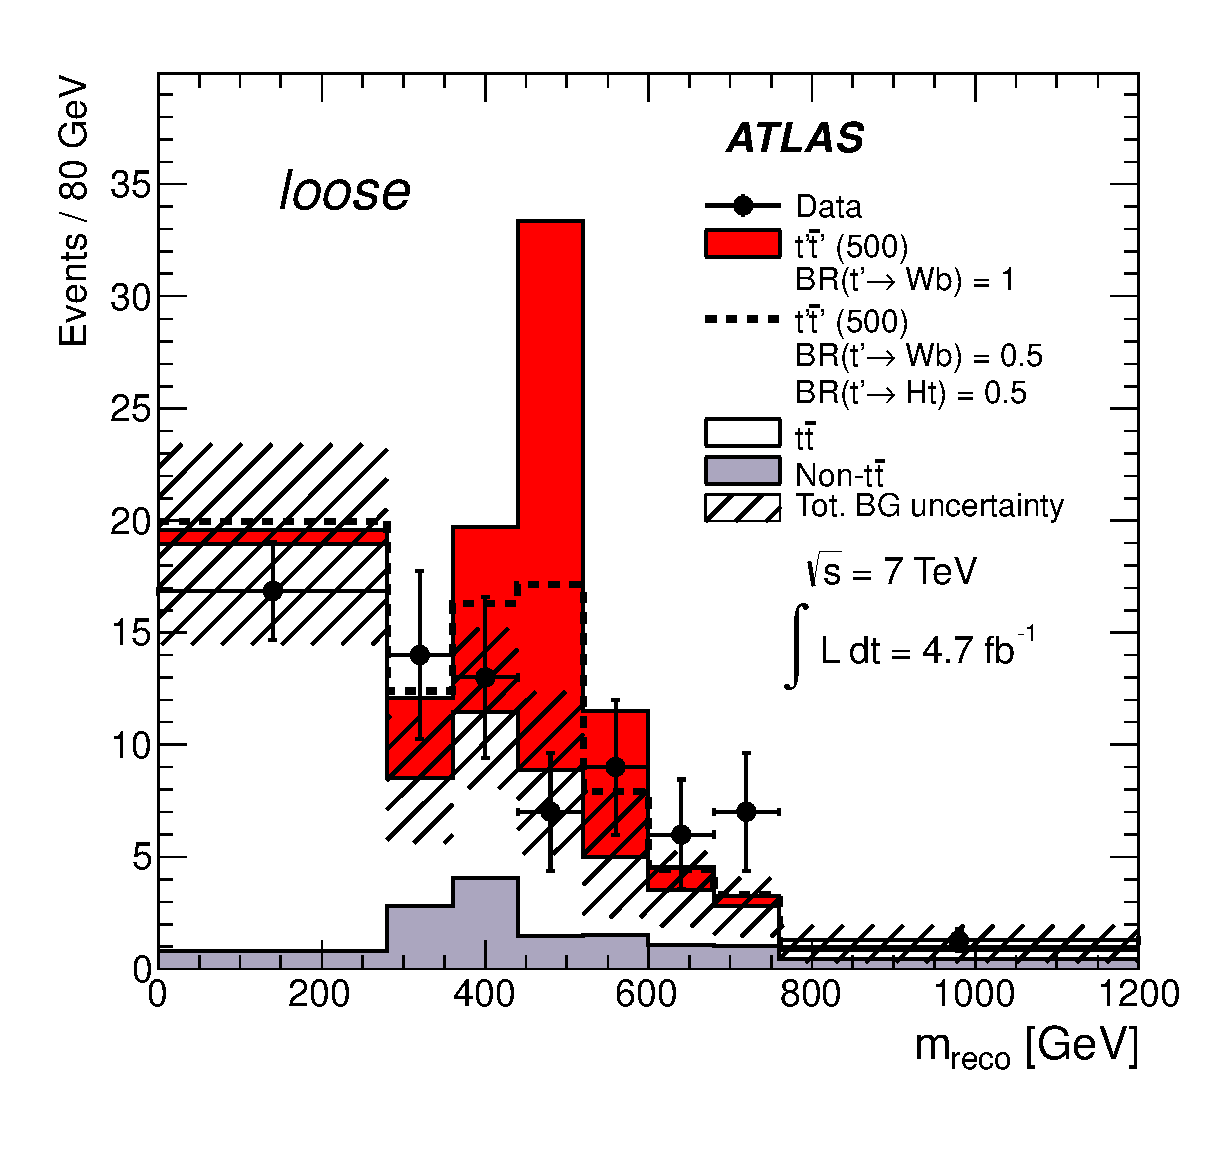
\includegraphics[width=0.45\textwidth]{appendices/figures/wbwb/fig_02a}}
  	%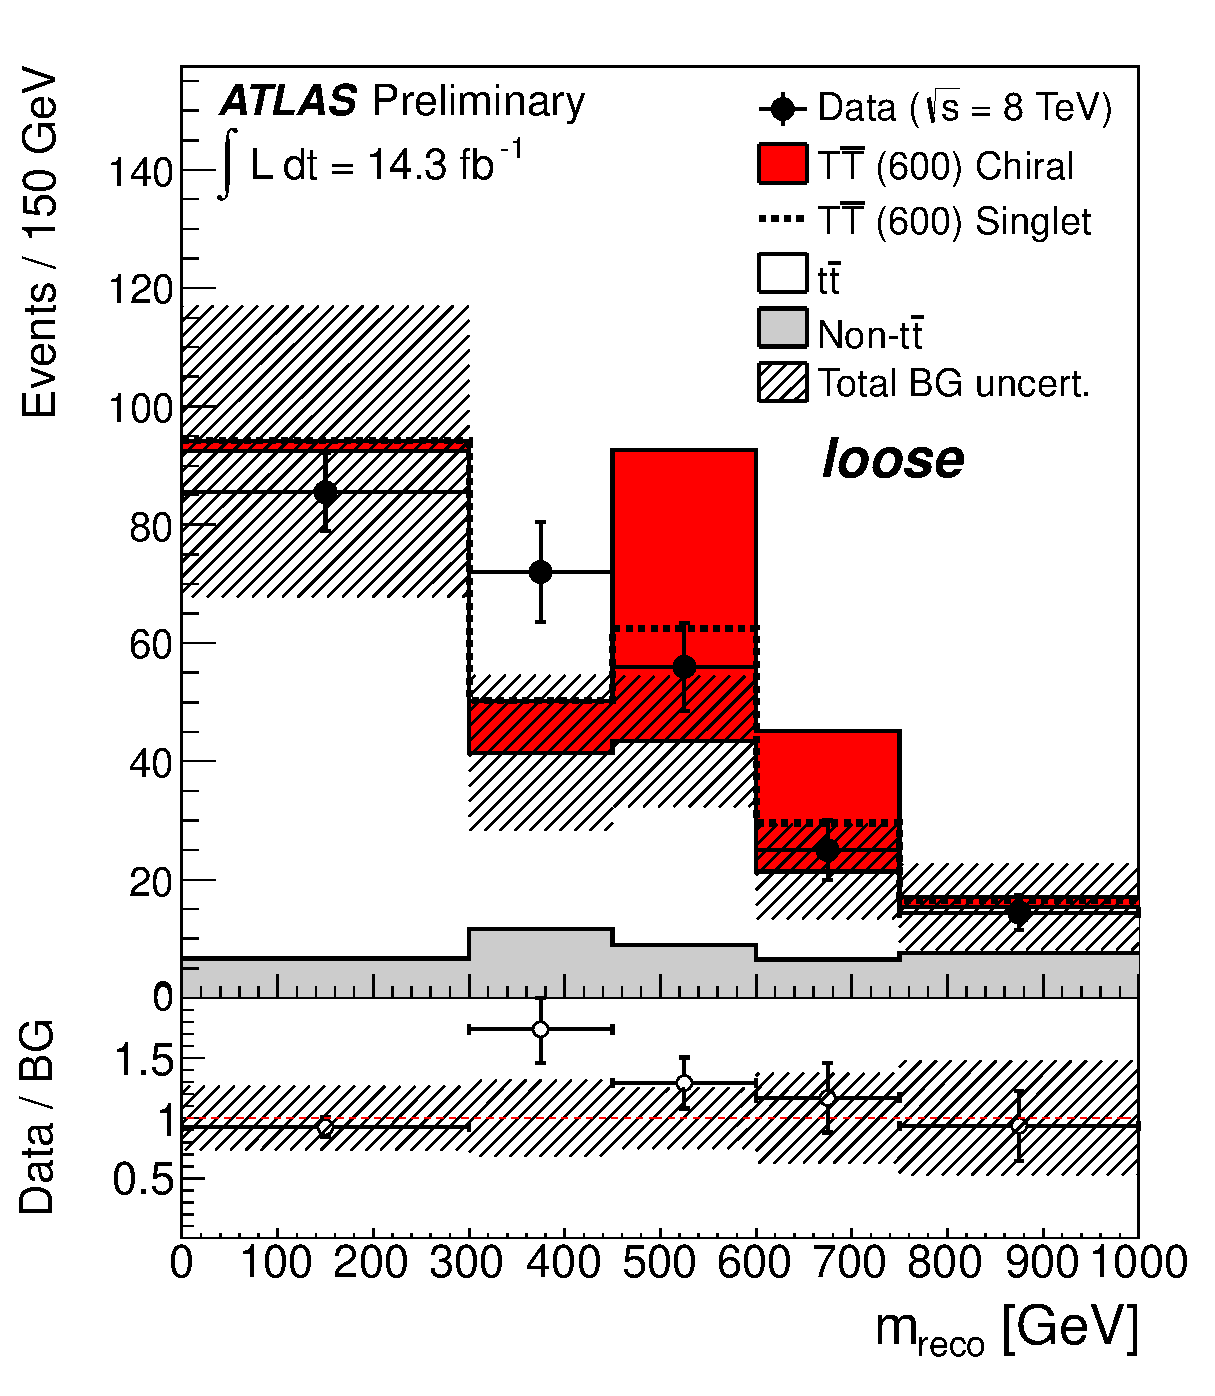
\includegraphics[width=0.45\textwidth]{wbx_analysis_14ifb/figures/confnoteplots/VLQAna_WbX_1W_MWb_4_ELEMUON_cutflow12345_NOMINAL.eps}}
	\subfigure[]{\label{fig:mrecoTIGHTBIS}
  	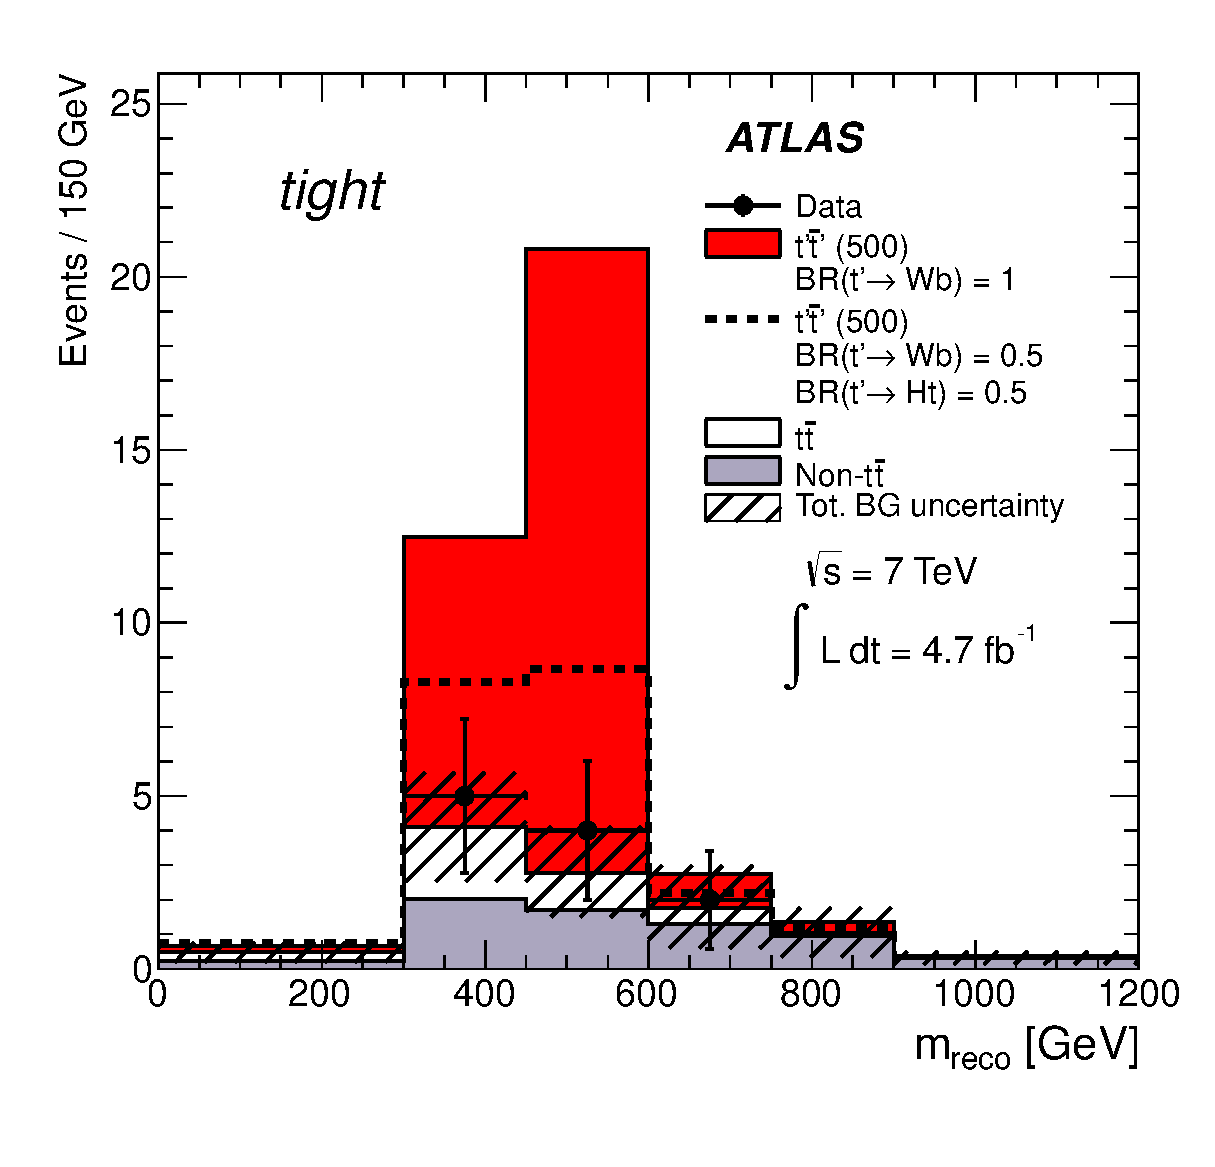
\includegraphics[width=0.45\textwidth]{appendices/figures/wbwb/fig_02b}}
  	%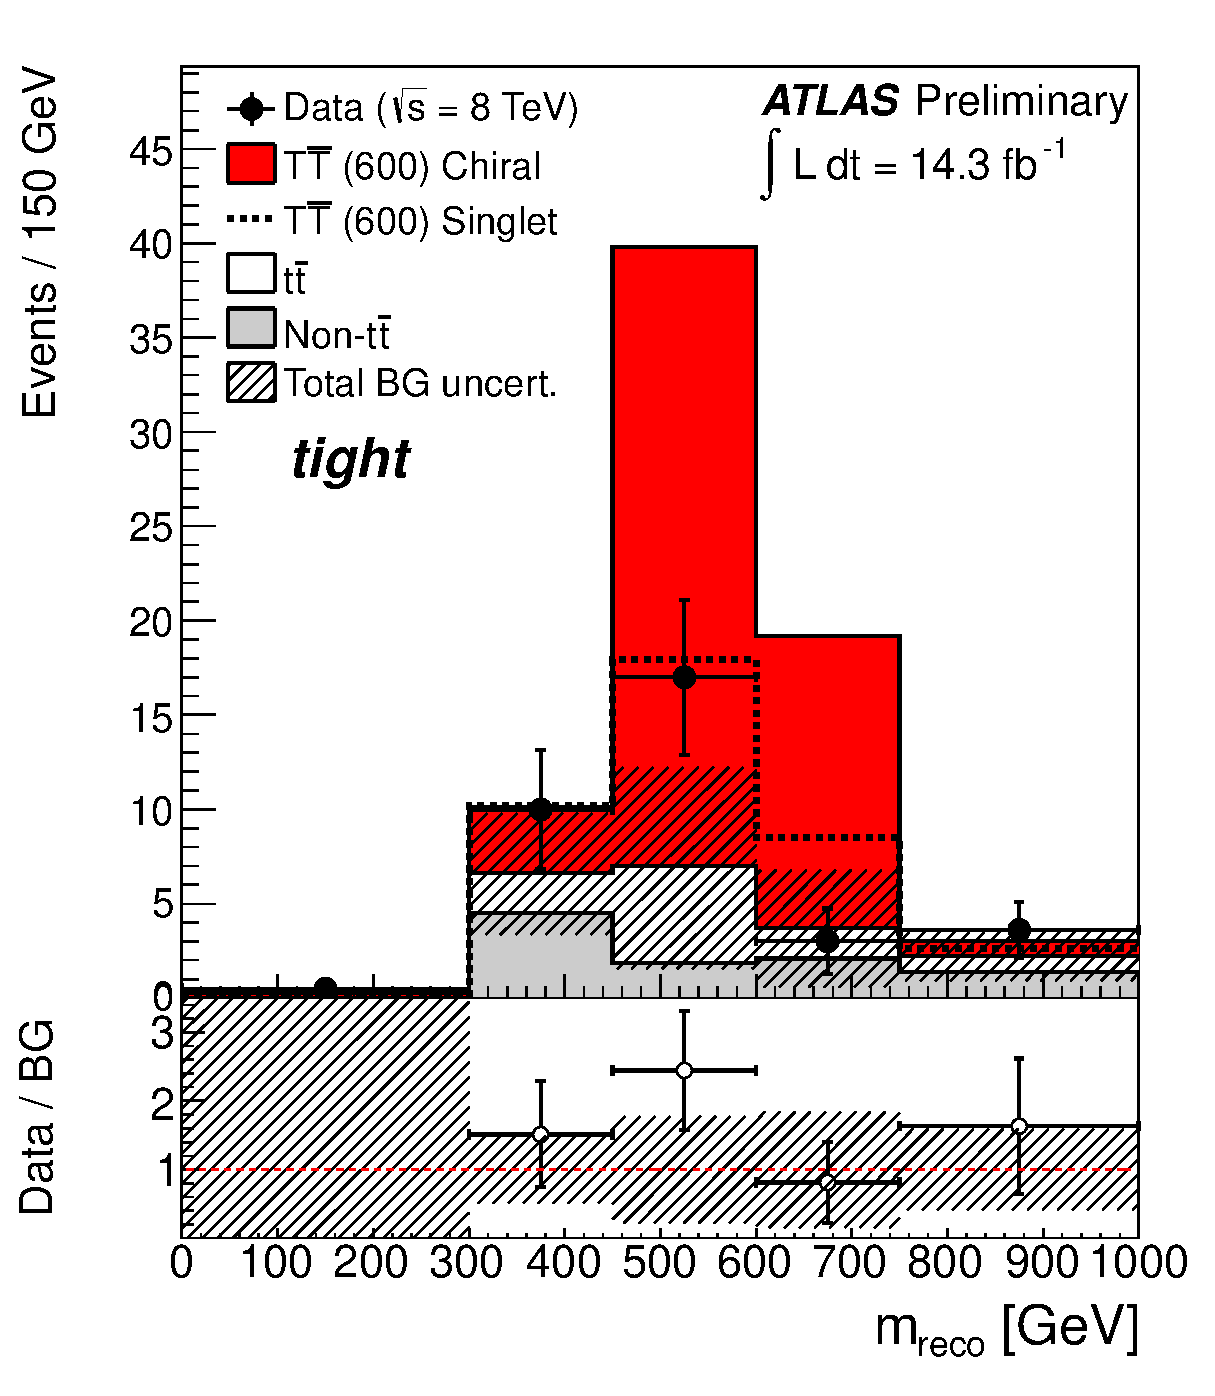
\includegraphics[width=0.45\textwidth]{wbx_analysis_14ifb/figures/confnoteplots/VLQAna_WbX_1W_MWb_4_ELEMUON_cutflow1234567_NOMINAL.eps}}
	\caption[bla]{Distribution of $m_{\rm reco}$  for the combined electron and muon channels after the (a) \loose\ and (b) \tight\ selection for the 7~\tev\ analysis.%        The data (solid black points) are compared to the background 
        prediction from Standard Model (stacked histograms). 
        The total uncertainty on the background estimation (see Section~\ref{sec:SystematicUncertainties} for details) is shown as a black hashed band.
        The expected contribution from a chiral fourth-generation 
        $\T$ quark with mass $m_{\T}=600\gev$ is also shown (red shaded histogram), 
        stacked on top of the Standard Model background. 
        The lower panel shows the ratio of data to Standard Model prediction. 
        The overflow has been added to the last bin.


        \label{fig:mrecoBIS}}
        %The shaded area represents the total background uncertainty (see Section~\ref{sec:SystematicUncertainties} for details). Also shown, stacked on top of the Standard Model background, is the expected contribution from signal corresponding to a chiral $\T$ quark with mass $m_{\T}=600\gev$.}
\end{center}\end{figure}

As can be seen in Figure~\ref{fig:cls_study}, the \tight\ configuration using 
\mreco\ distribution information achieves an expected
exclusion for a chiral fourth-generation $\T$ quark which is $\sim 50\gev$ 
higher than the reach of both the
\loose\ and \tight\ cut-and-count analyses, whose sensitivies are comparable.
Therefore, the \tight\ selection was chosen 
{\it a priori} to obtain the main result of the 7~\tev\ search.
The same argument is considered to hold for the \wbx\ analysis.

\begin{figure}[htb]\begin{center}
	\subfigure{
  	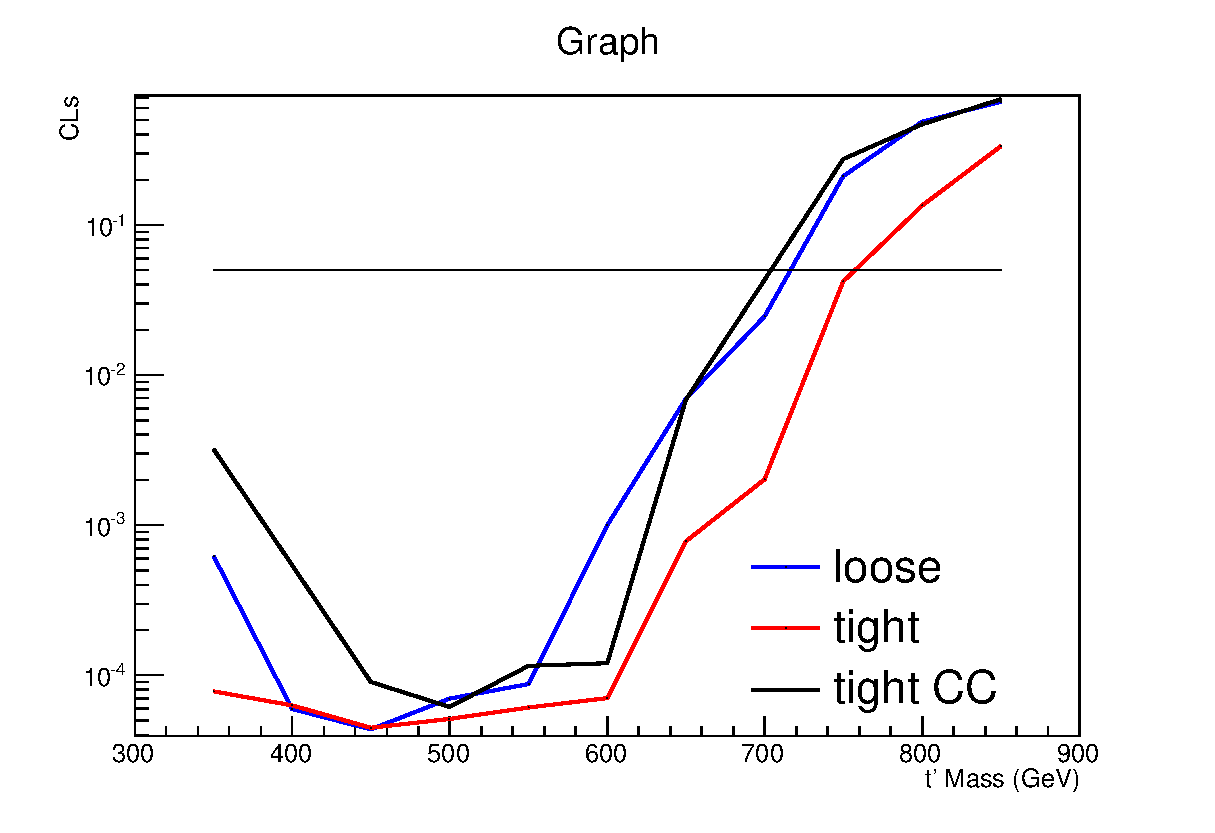
\includegraphics[width=0.7\textwidth]{results/figures/CLs_versus_Mass.eps}}
	\caption{Expected $CL_{\rm s}$ as a function of $m_{t'}$ taking into account systematic uncertainties.
Compared are three possible configurations for the 7~\tev\ analysis (see text for details).\label{fig:cls_study}}
\end{center}\end{figure}


